%%%%%%%%%%%%%%%%%%%%%%%%%%%%%%%%%%%%%%%%%%%%%%%%%%%%%%%%%%%%%%
%%%%		Informe de Canalizaciones
%%%%	Fecha	: Diciembre de 2020
%%%%	Autor	: Luis Millan
%%%%	Correo	: lmillan131@gmail.com
%%%%
%%%%%%%%%%%%%%%%%%%%%%%%%%%%%%%%%%%%%%%%%%%%%%%%%%%%%%%%%%%%%%

\documentclass[11pt,letterpaper]{article}
\usepackage[activeacute,spanish]{babel}
\usepackage[utf8]{inputenc}
\usepackage[letterpaper,includeheadfoot, top=0.5cm, bottom=3.0cm, right=2.0cm, left=2.0cm]{geometry}
\renewcommand{\familydefault}{\sfdefault}
\usepackage{graphicx}
\usepackage{color}
\usepackage{hyperref}
\usepackage{amssymb}
\usepackage{url}
\usepackage{fancyhdr}
\usepackage{hyperref}
\usepackage{subfig}
\usepackage{listings}
\usepackage{mathrsfs,amsmath}
\lstset{language=C, tabsize=4,framexleftmargin=5mm,breaklines=true}

% =============== Inicio de Documento =============== 
\begin{document}
% =============== Portada =============== 
\newpage
\pagestyle{fancy}
\fancyhf{}
\vspace*{6cm}
\begin{center}
\Huge  {Canalizaciones y Distribución}\\
\vspace{1cm}
\end{center}
\vfill
\begin{flushright}
\begin{tabular}{ll}
Autor: & Luis E. Millán U.\\
Profesor: & Ing. Jorge Crespo\\
& \today\\
& Caracas, Venezuela.
\end{tabular}
\end{flushright}

% =============== Encabezado y pie de Pagina ===============
\newpage
\pagestyle{fancy}
\fancyhf{}
%Encabezado
\fancyhead[L]{\rightmark}
\fancyhead[L]{\small \rm \textit{Sección \rightmark}}
\fancyhead[R]{\small \rm \textbf{\thepage}}
%Pie 
\fancyfoot[L]{\small \rm \textit{Br. L. Millán}}
\fancyfoot[R]{\small \rm \textit{Canalizaciones y Distribución}}
\renewcommand{\sectionmark}[1]{\markright{\thesection.\ #1}}
\renewcommand{\headrulewidth}{0.5pt}
\renewcommand{\footrulewidth}{0.5pt}
\tableofcontents
%==========================================%
%  MOTORES
%==========================================%
\newpage
\section{Información General}
\subsection{Objetivos}
\subsubsection{Objetivo Principal:}
Adquirir conocimientos y herramientas necesarias para realizar diseños e implementaciones de proyectos de canalizaciones eléctricas y distribución.
\subsubsection{Objetivos Especificos:}
\begin{itemize}
	\item Aprender la distribución de la electricidad desde la acometida hasta los circuitos ramales.
	\item Proteger los ciscuitos y balancear los tableros.
\end{itemize}
\subsection{Formato de Clases}
La dinamica de las Clases será tipo Forochat, los dias Lunes y Miercoles desde las 8:00 a las 10:00, las dudas seran solventadas durante la hora de clase a través del chat privado, exceptuando aquellas dudas que se considere muy importante podra ser planteada en el chat grupal.
\subsection{Metodo de Evaluación}

\begin{itemize}
	\item \textbf{Parcial 1:} $30\%$
	\item \textbf{Parcial 2:} $20\%$
	\item \textbf{Proyecto 1:} $30\%$ (Individual)
	\item \textbf{Proyecto 2:} $15\%$ (Individual)
	\item \textbf{Asignaciones:} $5\%$
\end{itemize}
\section{Clases}
\subsection{Clase 1 Lunes 23/11/2020}
\textbf{Introducción}
\subsubsection{Partes de un Proyecto:}
\begin{itemize}
	\item \textbf{1} introducción del proyecto a desarrollar. El objetivo y lo que se necesita.

	\item \textbf{2} ubicación - condiciones ambientales (características del terreno; altitud; temperatura; nivel ceraunico; valores de resistividad del suelo)

	\item \textbf{3} características de la instalación (alta/media/baja; si es un centro comercial/colegio/residencia, etc)
 
	\item \textbf{4} alcance: elementos que se deben desarrollar para cumplir los objetivos del proyecto)

	\item \textbf{5} Referencias (nacionales e internacionales) 

	\item \textbf{6} criterios en base a las referencias 

	\item \textbf{7} cálculos.

	\item \textbf{8} especificaciones (materiales al detalle, altura, posición, ubicación, tipo de tubería, etc).

	\item \textbf{9} planos

	\item \textbf{10} cómputos (indicar cantidades de lo que se necesita)

	\item \textbf{11} Partida (Norma covenin 2000)

	\item \textbf{12} Análisis de precios unitarios (APU)

	\item \textbf{13} Costos - Precio general de la obra
\end{itemize}

\subsubsection{Alcances}
Los alcances pueden ser generales o de cargas especiales:

\begin{itemize}
	\item Fuerza: bomba de agua, portón eléctrico, ascensor, A.A, Cerco eléctrico.
	\item Iluminación: Interior (residencial, comercial, oficinas, fábricas, accesos, estacionamientos),	exterior (vial, fachada, recreación, estacionamiento, peatonal, de seguridad), emergencia, deportiva, arquitectónica.
	\item tomas de corriente de uso general.
	\item cargas o salidas especiales.
	\item Sistemas de intercomunicación.
	\item Sistemas de tv por cable.
	\item Sistemas de puesta a Tierra
	\item sistema de teléfono.
	\item sistema de protección contra incendios.
	\item Sistema de protección contra descargas atmosféricas.
	\item Sistemas de vigilancia y seguridad.
\end{itemize}

\textbf{Nota:} Es importante las referencias en los proyectos, eso permite estar en norma respecto al país donde se desarrolle el proyecto y en caso que no exista regulación siempre tendrán las normas internacionales, nosotros nos regimos por el Código Eléctrico Nacional, el cual se basa en el NFPA de EEUU.\\
Actualmente existen normativas para cada etapa de los proyectos, entre las nacionales tenemos: Fondonorma / Covenin y CEN - Fondonorma 200.\\
Ej: Rayos - Fondonorma 599; Tensiones normalizadas - Fondonorma 159\\

Las internacionales son: IEEE, IEC, NFPA.
\subsection{Clase 2 Miércoles 25/11/2020}
\subsubsection{Selección de Conductores}
Criterio para la selección de Conductores:
\begin{itemize}
	\item \textbf{1} capacidad de corriente
	\item \textbf{2} caída de tensión.
	\item \textbf{3} capacidad de cortocircuito.
	\item \textbf{4} nivel de tensión.
	\item \textbf{5} fluctuaciones de tensión.
	\item \textbf{6} ambiente de instalación
\end{itemize}
\textbf{Nota:} La conexión en hogares viene de un banco de transformadores local a un elemento de protección o breaker y
 finalmente a los diferentes tableros que alimentan los circuitos.\\
 
\textbf{Nota:} Intentar evitar empalmes, cada empalme es un punto de posible sobrecalentamiento.\\

\textbf{Nota:} La ventaja del aluminio sobre el cobre es basicamente su precio y el peso y las desventaja es que el cobre tiene una mayor capacidad para transportar corriente.\\
 
La primera característica a tomar en cuenta es la clasificación de los calibres de los cables (AWG/kcmil), desde el cable 18 hasta el 0000 (4/0) se denota AWG, en adelante se utiliza kcmil.\\

En baja tensión en aspectos residenciales normalmente se utilizan:

\begin{itemize}
	\item Cable 18 para control.
	\item Cable 12 tomas e iluminación.
	\item Cable 10 aires y cargas especiales.
	\item Cable 8 (secadoras, aires y cargas especiales)
	\item Cable 6 (acometidas)
\end{itemize}

\textbf{Nota:} Es importante la chaqueta según el ambiente en el que se vaya a trabajar. Existen chaquetas que soportan intemperie, agua, aceite, humedad, etc. Algunas chaquetas como la ttu y la thhn son robustas para evitar su fractura al ser cableadas o pasadas por tubos.\\

\textbf{Nota:} Cuando la temperatura del cable supera el límite permisible el aislante comienza a derretirse, si es fase activa es muy probable que haga contacto con otro cable o tubería y ¡EXPLOTA EL CABLE!\\

\textbf{Nota Secreto:} De manera general los fabricantes diseñan los cables cuidando un margen de seguridad. A los valores vistos normalmente el cable soporta hasta un 15$\%$ por encima de su valor.\\

Tenemos que considerar la temperatura ambiente, no es lo mismo dejar un cable a la intemperie en Maracaibo, en Mérida o en caracas, para una temperatura entre 26-30° el factor es 1, para Maracaibo que está como entre 36-40 (0,82).

\textbf{Nota:} De manera general se recomienda siempre trabajar con tres conductores portadores de corriente. Sin embargo, hay ocasiones en que hay que añadir una 4ta fase. Al agregar la 4ta fase, las características del conductor se reducen un 80$\%$ cómo lo establece la tabla 310.15\\

\begin{figure}[ht!]
	\centering
	\fbox{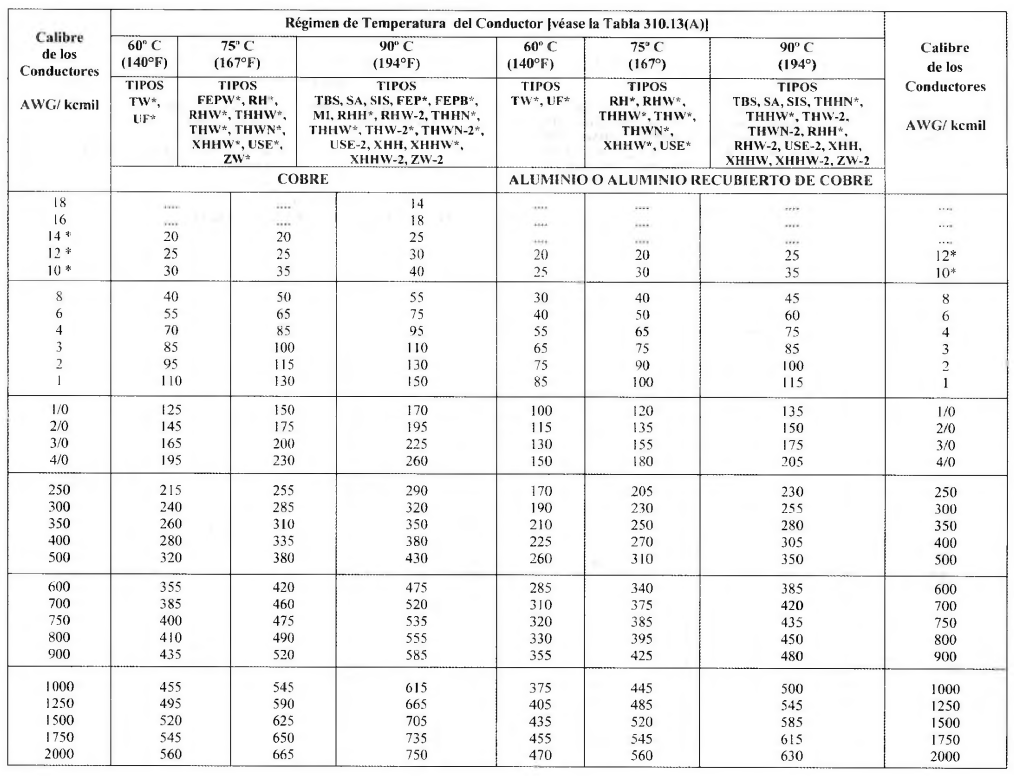
\includegraphics[scale=0.4]{310.16.png}}
	\caption{Ampacidades Admisibles de los Conductores Aislados para tensiones nominales (310.16)}
\end{figure}

\begin{figure}[ht!]
	\centering
	\fbox{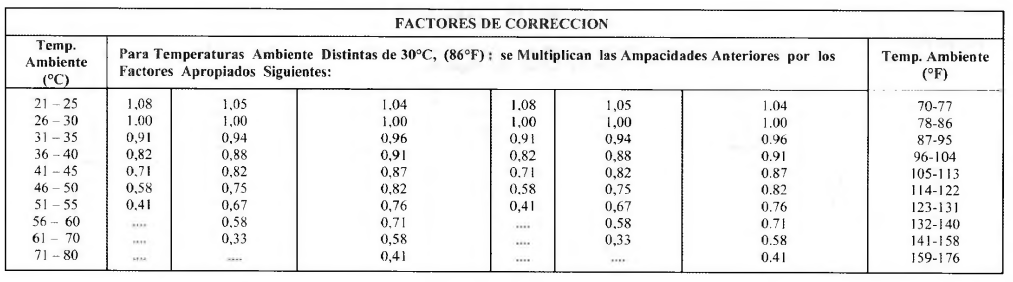
\includegraphics[scale=0.4]{310.16_correcciones.png}}
	\caption{Factor de Corrección para 310.16}
\end{figure}

\subsection{Clase 3 Miércoles 4/12/2020}
	Es importante aprender a distribuir la carga en un tablero. De aquí en adelante solo deben ampliar la cantidad de circuitos en función del tablero que seleccionen o de la cantidad de cargas que vayan a manejar, un tablero de 4 hilos normalmente es 3 fases y neutro y uno de 5 hilos es 3 fases, neutro y tierra.
	
\subsubsection{Breakers}	

Los breaker normalmente termomagnéticos se seleccionan para proteger el cable de nuestro circuito. Debe ser seleccionado a un valor inmediato menor al establecido en la tabla 310.16 del CEN. Se pueden guiar de la sección 240.6.\\

Hay dos tipos fundamentales de breakers: Enchufables y Superficiales; los enchufables se consiguen normalmente en tableros de dos fases residenciales (embutidos).\\

Los breaker son clasificados por polos, por ejemplo:

\begin{itemize}
	\item Breaker 1x20A (de un solo polo).
	\item Breaker 2x50A (de dos polos).
	\item Breaker 3x225A (tres polos).
\end{itemize}

	\textbf{Regímenes de Corriente Normalizados (240.6):} Fusibles e Interruptores Automáticos de Caja Moldeada. Los regímenes de corriente normalizados de los fusibles e interruptores automáticos de caja moldeada de tiempo, inverso, serán de 15, 20, 25, 30, 35,40,45, 50, 60, 70, 80, 90, 100,110,125,150,175,200,225,250,300,350,400,450,500, 600, 700, 800,1.000,1.200, 1.600, 2.000, 2.500, 3.000,4.000, 5.000 y 6.000 A.\\
	Adicionalmente, como régimen normalizado de los fusibles se considerará las de 1,3,6, 10 y 601 A. Se permitirá el uso de fusibles e interruptores automáticos de tiempo inverso con un régimen de corriente que no esté normalizado.

\subsubsection{Ejercicio Nº1}

Para los siguientes elementos, seleccione el cable que usarían para alimentar todo y realice el balanceo en un tablero, verifique los consumos:

\begin{itemize}
	\item 15 lámparas 100w @120v fp=1.
	\item 5 lámparas 600w @208V fp 0,8.
	\item Un aire acondicionado que consume 17A trifásicos.
\end{itemize}
Los pasos para la solución son los siguientes:
\begin{enumerate}
	\item Calculas con la potencia la corriente del circuito ramal.

	\item seleccionas el cable según 310.16.

	\item seleccionas la protección.
\end{enumerate}

Necesitamos saber la corriente que consumirá cada carga. En el caso de las lámparas y los equipos no sabemos, el de los aires si.

	
\section{Asignaciones}
\subsection{Asignación 1 Miercoles 25/11/2020}
\textbf{Niveles de Tensión en Venezuela}
Segun el informe publicado el 16 de julio del 2020 con titulo: "INFORME DE COMISIÓN DE TRANSMISIÓN ELÉCTRICA", del Portal de Asociación Venezolana de Ingenieros Electricistas, Mecánicos y Profesiones Afines (AVIEM), los niveles de tensión en venezuela son: 69 kV; 115 kV; 138 kV; 230 kV; 400 kV y 765 kV.

Portal: \url{https://aviem.org/informe-de-comision-de-transmision-electrica/#:~:text=Los%20niveles%20de%20tensi%C3%B3n%20utilizados,400%20kV%20y%20765%20kV.}


\subsubsection{Retroalimentación}
\textbf{Nota:} Normalmente todos los centros comerciales realizan la distribución en 480V y cada local tiene un trx para tener nuestro servicio 208/120, esto facilita la alimentación de los chiller, ascensores y la distribución de la energía con una mayor eficiencia.\\

\subsection{Asignación 2 Lunes 30/11/2020}
\textbf{Tipos de Tableros de Distribución, Cantidad de Circuitos y Características y Plano de Casa}

	Los tableros eléctricos prácticamente son armazones metálicos que se utilizan para proteger a todos los componentes de mando y de control de cualquier sistema eléctrico, ya sea desde un circuito básico de un hogar hasta los componentes de uno más complejo como el de una máquina industrial.

\begin{figure}[ht!]
	\centering
	\fbox{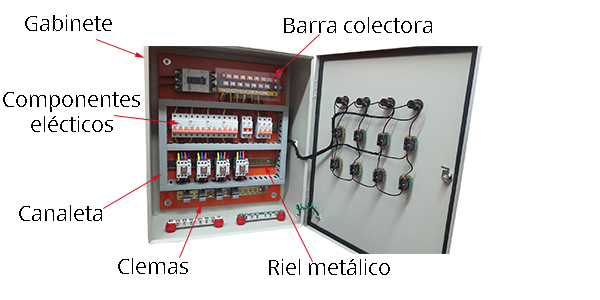
\includegraphics[scale=2]{Partes-tablero.jpg}}
	\caption{Partes de un Tablero}
\end{figure}
\subsubsection{Tipos de Tableros}
\begin{itemize}
	\item \textbf{Panel de Distribución para Circuitos Ramales de Alumbrado y de Artefactos}\\
	 Un panel de distribución para circuitos ramales de alumbrado y de artefactos es aquel que tiene más de un 10 por ciento de sus dispositivos de protec­ción de sobrecorriente de 30 amperios o menos protegiendo circuitos ramales de alumbrado y de artefactos.
	 
	\item \textbf{Panel de Distribución de Potencia}\\
 Un panel de distri­bución de potencia es aquel, que tiene el 10$\%$ o menos de sus dispositivos de protección de sobrecorriente protegiendo circuitos ramales de alumbrado y de artefactos.
 
	\item \textbf{Tablero Eléctrico para Uso en Viviendas}\\
 Un tablero eléctrico para uso en viviendas es similar a un panel para alumbrado y artefactos, pero de máximo 250 voltios y equipado exclusivamente con interruptores automáticos en caja moldeada del tipo insertable.
 
 	\item \textbf{Tablero de Control Industrial} U ensamble de dos o más componentes consistente de uno de los siguientes:
 	\begin{enumerate}
 		\item Solamente componentes de circuitos de potencia, tales como controladores de motores, relés de sobrecarga, suiches y seccionadores con fusibles e interruptores automáticos.
 		
 		\item Solamente componentes de circuitos de control, tales como pulsadores, luces pilotos, selectores, temporiza- dores, suiches, relés de control, etc.
 		
 		\item Una combinación de componentes de circuitos de potencia y de control.
 	\end{enumerate}
 	Esos componentes, juntos con el cableado y los terminales, están montados sobre o dentro de una envolvente o montados sobre un panel auxiliar. El tablero de control industrial no incluye los equipos controlados.
\end{itemize}
\subsubsection{Circuitos Ramales}
Los circuitos ramales comprendidos en esta Sección se clasificarán de acuerdo con la capacidad de corriente nominal o el máximo valor de ajuste permitido del dispositivo de sobrecorriente. La clasificación de los circuitos ramales que no sean individuales será de 15,20, 30, 40 y 50 A. Cuando por cualquier razón se utilicen conducto­res de mayor capacidad, la capacidad nominal o ajuste del dispositivo de sobrecorriente especificado determinará la clasificación del circuito.

\begin{figure}[ht!]
	\centering
	\fbox{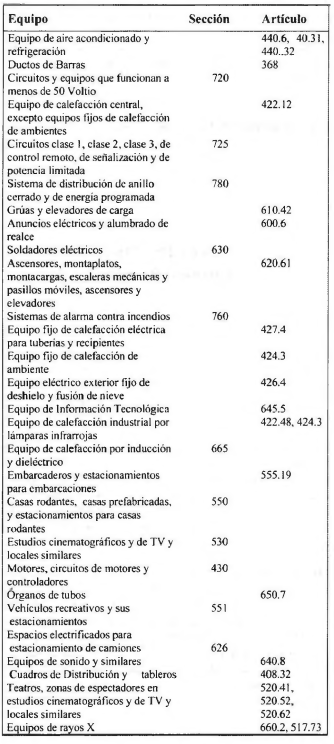
\includegraphics[scale=0.7]{210.2.png}}
	\caption{Circuitos Ramales para uso específico}
\end{figure}

\newpage
\textbf{Circuitos Ramales Necesarios} Los circuitos ramales para iluminación y aparatos, incluyendo los aparatos operados con motor serán provistos para suministrar las cargas calculadas según el Cálculo de Cargas del Circuito Ramal (220.10). Adicionalmente, los circuitos ramales serán provistos para cargas específicas no cubiertas por dicho cálculo donde sea requerido en cualquier parte de este Código y para cargas para unidades de vivienda según el Cálculo de Cargas del Circuito Ramal (220.10).
\begin{itemize}
	\item \textbf{Número de Circuitos Ramales} El número mínimo de circuitos ramales se determinará a partir de la carga total calculada y del tamaño o capacidad de los circuitos utilizados. En todas las instalaciones, el número de circuitos será el adecuado para alimentar la carga servida. En ningún caso, la carga de un circuito excederá la máxima especificada en la sección de Cargas Máximas (220.18).

	\item \textbf{Carga Proporcionalmente Repartida Entre los Circui­tos Ramales} Cuando la carga se calcula con base a voltioamperios por metro cuadrado, el sistema de cableado resultante, incluyendo los tableros para los circuitos ramales se proveerán para alimentar como mínimo la carga calculada. Esta carga será proporcionalmente repartida dentro de los circuitos ramales para salidas múltiples en los tableros. Los elementos de protecciones de los circuitos ramales y circuitos serán requeridos únicamente para servir las cargas conectadas.

	\item \textbf{Unidades de Viviendas}
		\begin{enumerate}
			\item \textbf{Circuitos Ramales para Pequeños Aparatos} En adición al número de circuitos ramales requeridos en otros sitios de este Artículo, dos o mas circuitos ramales de 20 A serán provistos para los tomacorrientes especificados en la seccion de Salidas para Tomacorrientes en Unidades de Vivienda (210.52).
			\item \textbf{Circuitos Ramales para Lavanderías} En adición al número de circuitos ramales requeridos en otros sitios de este Artículo, por lo menos un circuito ramal adicional de 20 A será provisto para el (los) tomacorriente(s) especifícado(s) en la seccion de Salidas para Tomacorrientes en Unidades de Vivienda (210.52). Este circuito no tendrá otras salidas.
			\item \textbf{Circuitos Ramales de Salas de Baño} En adición al número de circuitos ramales requeridos en otros sitios de este Artículo, al menos un circuito ramal de 20 A será provisto para el (los) tomacorriente(s) de la sala de baño. Este circuito no tendrá otras salidas.
		\end{enumerate}
\end{itemize}
\subsubsection{Retroalimentación}
Otra forma de categorizar los tableros de distribución es la siguiente:
\begin{enumerate}
	\item 	\textbf{Tableros de Alumbrado Tipo NLAB}\\
		Este tablero es utilizado generalmente para la protección y corte de circuitos de iluminación, tomacorrientes y carga menores tales como: pequeños equipos de aire acondicionado, máquinas de oficinas y otros.Características Eléctricas
		\begin{itemize}
			\item \textbf{Barras Principales:} 125 hasta 400 Amp. Máxima.
			\item \textbf{Interruptor Principal:} con o sin (400Amp. Máxima).
			\item \textbf{Interruptores modelo:} Cutler Hammer, Square D, General Electric, ABB.
			\item \textbf{Voltaje de trabajo:} 240/120 Vac. Máxima 60 Hz.
			\item \textbf{Servicio:} 2 Fases 3 Hilos | 2 Fases 4 Hilos | 3 Fases 4 Hilos | 3 Fases 5 Hilos.
			\item \textbf{Montaje:} Superficial o Empotrado, Intemperie o a Prueba de Polvo.
			\item \textbf{Número de Circuitos:} Hasta 42 circuitos.
			\item \textbf{Barras:} Plateadas ó Pintadas.
			\item \textbf{Capacidad de Interrupción Máxima:} 10KA Icc (rms) en 240 VAC. Limitados por los circuitos Ramales.
			\item \textbf{Lámina utilizada:} Calibre 16 (1.5mm) Calibre 14 (1.9mm).
			\item \textbf{Pintura:}	Gris Electrostatico RAL 7042.
		\end{itemize}
	
	\item \textbf{Tableros de Alumbrado y Distribución Tipo NAB}\\
		Este tablero es utilizado para la protección y corte de circuitos de iluminación y pequeñas cargas de alimentadores que posteriormente son protegidos por los otros dispositivos tales como: guardamotores, seccionadores y otros. Normalmente  alimentan circuitos ramales de: maquinas pequeñas de potencias y/o sub tableros.
		\begin{itemize}
			\item \textbf{Barras Principales:} 600 Amp. Máxima.
			\item \textbf{Interruptor Principal:} con o sin (600Amp. Máxima).
			\item \textbf{Interruptores modelo:} Cutler Hammer, Square D, General Electric, ABB.
			\item \textbf{Voltaje de trabajo:} 208/120 Vac. Máxima 60 Hz.
			\item \textbf{Servicio:} 2 Fases 3 Hilos | 2 Fases 4 Hilos | 3 Fases 4 Hilos | 3 Fases 5 Hilos.
			\item \textbf{Montaje:} Superficial o Empotrado, Intemperie o a Prueba de Polvo.
			\item \textbf{Número de Circuitos:} Hasta 42 circuitos.
			\item \textbf{Barras:} Plateadas ó Pintadas.
			\item \textbf{Capacidad de Interrupción Máxima:} 14KA Icc (rms) en 240 VAC.
			\item \textbf{Lámina utilizada:} Calibre 16 (1.5mm) Calibre 14 (1.9mm).
			\item \textbf{Pintura:} Gris Electrostatico RAL 7042.
		\end{itemize}
	
	\item \textbf{Tableros de Alumbrado y Distribución Tipo NHB}\\
		Este tablero es utilizado para la protección y corte de circuitos de iluminación, cargas de alimentadores, alumbrado, maquinas y sub tableros.
		\begin{itemize}
			\item \textbf{Barras Principales:} 600 Amp. Máxima.
			\item \textbf{Interruptor Principal:} con o sin (600Amp. Máxima).
			\item \textbf{Interruptores modelo:} Cutler Hammer, Square D, General Electric, ABB.
			\item \textbf{Voltaje de trabajo:} 480/277 Vac. Máxima 60 Hz.
			\item \textbf{Servicio:} 2 Fases 3 Hilos | 2 Fases 4 Hilos | 3 Fases 4 Hilos | 3 Fases 5 Hilos.
			\item \textbf{Montaje:} Superficial o Empotrado, Intemperie o a Prueba de Polvo.
			\item \textbf{Número de Circuitos:} Hasta 42 circuitos.
			\item \textbf{Barras:} Plateadas ó Pintadas.
			\item \textbf{Capacidad de Interrupción Máxima:} 25KA Icc (rms) en 480 VAC. 18 KA Icc (rms) 600 VAC.
			\item \textbf{Lámina utilizada:} Calibre 16 (1.5mm) Calibre 14 (1.9mm).
			\item \textbf{Pintura:} Gris Electrostatico RAL 7042.
		\end{itemize}
	
	\item \textbf{Tableros de Fuerza y Distribución Tipo CCB}\\
		Este tablero es utilizado para la protección y corte de circuitos de iluminación y pequeñas cargas de alimentadores que posteriormente son protegidos por los otros dispositivos tales como: guardamotores, seccionadores y otros. Normalmente  alimentan circuitos ramales de: maquinas pequeñas de potencias y/o sub tableros.
		
		\begin{itemize}
			\item \textbf{Barras Principales con Principal:} 1200 Amp. Máxima.
			\item \textbf{Barras Principales sin Principal:} 2000 Amp. Máxima.
			\item \textbf{Interruptores modelo:} Cutler Hammer, Square D, General Electric, ABB.
			\item \textbf{Voltaje de Trabajo y Voltaje de Aislamiento:} 600 Vac. Máxima 60 Hz.
			\item \textbf{Servicio:} 3 Fases 4 Hilos | 3 Fases 5 Hilos.
			\item \textbf{Montaje:} Autosoportado.
			\item \textbf{Número de Circuitos:} Según requerimientos, con disposición y requisición de los clientes. De los elementos de distribución horizontal no más de 42 circuitos (según norma COVENIN 0542-1999).
			\item \textbf{Barras:} Desnudas o con Recubrimiento Aislante, Plateadas ó Pintadas.
			\item \textbf{Capacidad de Interrupción Máxima:} 65KA Icc (rms) en 240 VAC.
			\item \textbf{Cubierta o Ejecución:}
				\begin{enumerate}
				 	\item A prueba de polvo y agua (Nema 12).
				 	\item Para uso a la intemperie (Nema 3R)
				 	\item Para ambiente corrosivo (Nema 4X)
				\end{enumerate}
			\item \textbf{Lámina utilizada:} Calibre 14 (1.9mm).
			\item \textbf{Pintura:} Gris Electrostatico RAL 7042.
		\end{itemize}
	\item \textbf{Tableros de Distribución de Potencia Tipo CDP}\\
		Utilizado mayormente para la distribucion principal desde la Sub-estacion a los diferentes centros de carga y/o Sub – Alimentadores de la mayoria de los casos, conteniendo instrumentos tales como: voltimetro, amperimetros, kilovatimetros, kilovatrimetros horas, cosfimetro, selectores de fases, entre otros. Igualmente suelen contener relés de protección por falla de fase, falla a tierra, señalizacion de averias y otros.
		\begin{itemize}
			\item \textbf{Barras Principales con Principal:} Hasta 4000 Amp. Normalmente.
			\item \textbf{Interruptor Principales:} 4000 Amp. Máxima.
			\item \textbf{Interruptores modelo:} Cutler Hammer, Square D, General Electric, ABB.
			\item \textbf{Voltaje de Trabajo y Voltaje de Aislamiento:} 600 Vac. Máxima 60 Hz.
			\item \textbf{Servicio:} 3 Fases 4 Hilos | 3 Fases 5 Hilos.
			\item \textbf{Montaje:} Autosoportados.
			\item \textbf{Tipo de Construcción:} Con o sin compartimientos.
			\item \textbf{Número de Circuitos:} Según requerimientos
			\item \textbf{Barras:} Plateadas ó Pintadas.
			\item \textbf{Capacidad de Interrupción Máxima:} 120KA Icc (rms) en 600 VAC. Máxima.
			\item \textbf{Cubierta o Ejecución:} 
				\begin{enumerate}
					\item A prueba de polvo y agua (Nema 12).
					\item Para uso a la intemperie (Nema 3R).
					\item Para ambiente corrosivo (Nema 4X).
				\end{enumerate}
			\item \textbf{Lámina utilizada:} Calibre 14 (1.9mm).
			\item \textbf{Pintura:} Gris Electrostatico RAL 7042.
		\end{itemize}
	\item \textbf{Centros de Control de Motores CCM}\\
		Un Centro  Control de motores ó C.C.M. por definicion es un arreglo de varias unidades agrupadas para proteger un determinado grupo de motores, como tambiém permite lograr a través de su cableado interior el automatismo para realizar un determinado proceso, la ventaja que ofrece este sistema es que permite tanto la supervisión como la operación con un minimo costo.\\	
Las unidades de protección y corte de circuito pueden ser: interruptores termomagnéticos o fusibles para protección de motores. Los guardamotores o arrancadores podrán ser de protección térmica fija o ajustable, como también podrán ser con compensación de temperatura ambiental o no.\\
Este tipo de equipos, es conocido como fijo por contar con 02 compartimientos provisto de doble fondo, en donde una sección se encuentran alojados los equipos de control de arrancadores, relés térmicos y pulsadores, en la otra sección se encuentra un chasis con un sistema de barras de cobre el cual depende de la cantidad de arrancadores a servir.
		\begin{itemize}
			\item \textbf{Barras Principales con Principal:} 4000 Amp. Normalmente.
			\item \textbf{Interruptor Principal:} 4000 Amp. Máxima.
			\item \textbf{Arrancadores modelo:} Cutler Hammer, Square D, General Electric, ABB.
			\item \textbf{Voltaje de Trabajo:} 600 Vac. Máxima 60 Hz.
			\item \textbf{Voltaje de Aislamiento:} 600 Vac. Minimo 60 Hz.
			\item \textbf{Voltaje de Control:} 120 VAC. 60Hz.
			\item \textbf{Servicio:} 3 Fases 4 Hilos | 3 Fases 5 Hilos.
		 	\item \textbf{Montaje:} Autosoportado.
			\item \textbf{Barras:} Desnudas o con Recubrimiento Aislante, Plateadas ó Pintadas 
			\item \textbf{Capacidad de Interrupción Máxima:} 65KA Icc (rms) en 240 VAC.
			\item \textbf{Cubierta o Ejecución:}
			\begin{enumerate}
				\item A prueba de polvo y agua (Nema 12).
				\item Para uso a la intemperie (Nema 3R).
				\item Para ambiente corrosivo (Nema 4X).
			\end{enumerate}
			\item \textbf{Lámina utilizada:} Calibre 14 (1.9mm).
			\item \textbf{Pintura:} Gris Electrostatico RAL 7042 ó 7032.		
		\end{itemize}
	\item \textbf{Arrancadores}\\
		Este tablero es empleado con una combinación de contactor y relé térmico para el arranque de motores, incluye elementos de supervisión, control y mando.
		\begin{itemize}
			\item \textbf{Voltaje de trabajo:} Hasta 600 VAC. 60Hz.
			\item \textbf{Voltaje de Control:} 120 VAC. 60Hz.
			\item \textbf{Servicio:} 3 Fases 4 Hilos | 3 Fases 5 Hilos.
			\item \textbf{Montaje:} Superficial, Intemperie o a Prueba de Polvo.
			\item \textbf{Lámina utilizada:} Calibre 16 (1.5mm) Calibre 14 (1.9mm).
			\item \textbf{Pintura:} Gris Electrostatico RAL 7042 ó 7032.
		\end{itemize}
	\item \textbf{Tableros de Aislamiento Uso Hospitalario}
		Estos tableros estan diseñado para uso Hospitalario en aréas de Observación, Quirófano, Unidad de Cuidados Intensivos entre otros. Su objetivo principal es detectar fallas a tierras de Equipos Conectados al mismo para así evitar riesgos eléctricos que atenten contra la vida del paciente.
		\begin{itemize}
			\item \textbf{Barras Principales:} Hasta 400 Amp.
			\item \textbf{Interruptor Principal:} Hasta 225Amp.
			\item \textbf{Tansformador de Aislamiento:} 3KVA | 5KVA | 7.5KVA | 15KVA | 25KVA.
			\item \textbf{Voltaje de Operacion:} 120/208/240 Vac. Máxima 60 Hz.
			\item \textbf{Servicio:} 1 Fase 3 Hilos | 2 Fases 4 Hilos | 3 Fases 5 Hilos.
			\item \textbf{Montaje:} Superficial o Embutido.
			\item \textbf{Número de Circuitos:} Hasta 42 circuitos.
			\item \textbf{Barras:} Plateadas ó Pintadas.
			\item \textbf{Nivel de Aislamiento:} 5mA.
			\item \textbf{Monitor de Aislamiento:} 120VAC | 240VAC.
			\item \textbf{Lámina utilizada en Caja:} Calibre 16 (1.5mm) en Hierro Negro Pulido.
			\item \textbf{Lámina utilizada en Puerta:} Calibre 16 (1.5mm) en Acero Inoxidable.
			\item \textbf{Pintura de la Caja:} Gris Electrostatico RAL 7042.
		\end{itemize}
	\item \textbf{Tomas para Uso Hospitalario}\\
		Son cajas en lámina calibre 16 uso empotrable que contendrá el número de tomas 120V y 220V requeridas según el uso, ademas de una toma tipo PLUG para aterramiento todos estos equipos son exclusivos para uso hospitario montados sobre una tapa en Acero Inoxidable. Generalmente instaladas en UCI (Unidad de Cuidados Intensivos) y Quirofanos.
		\begin{itemize}
			\item \textbf{Voltaje de trabajo:} 120/240 Vac.
			\item \textbf{Montaje:} Empotrado.
			\item \textbf{Lámina utilizada:} Calibre 16 (1.5mm) Acero Inoxidable.
		 	\item \textbf{Usos:} Unidad de Cuidados Intensivos y Quirofanos, entre otros.
		\end{itemize}
		
	\item \textbf{Transferencias Automaticas y Manuales}\\
		Estos dispositivos supervisan las fuentes de energía normal generado por una empresa distribuidora de Energía y una fuente de Energía de Emergencia generada por una platan ó generador, en caso de interrupción ó perdida de la energía normal el dispositivo electrónico del tablero envia señales de control para activar relé que accionarán el mecanismo de los interruptores y transferiran automaticamente los circuitos de la carga a la fuente de emergencia; una vez se haya restituido la energía primaria el proceso se invierte automaticamente.
		\begin{itemize}
			\item \textbf{Intensidad o Carga de Trabajo:} Manuales (160Amp a 1600Amp) ó Automaticas (250Amp a 1600Amp).
			\item \textbf{Marcas Modelo:} Telergon, ABB, Socomec.
			\item \textbf{Voltaje de trabajo:} 240/440/480 Vac. 60 Hz.
			\item \textbf{Montaje:} Superficial o Autosoportado.
			\item \textbf{Lámina utilizada:} Calibre 16 (1.5mm) Calibre 14 (1.9mm).
			\item \textbf{Pintura:} Gris Electrostatico RAL 7042.
		\end{itemize}
	\item \textbf{Consolas de Control y Mando}\\
		Estos equipos son usados generalmente para el control a distancia de arrancadores en plantas procesadoras que requieren de supervisión y control por parte de un operario; normalmente se utilizan en plantas Azucareras, Arroceras entre otras.
		\begin{itemize}
			\item \textbf{Montaje:} Autosoportado.
			\item \textbf{Lámina utilizada:} Calibre 16 (1.5mm) Calibre 14 (1.9mm).
			\item \textbf{Pintura:} Gris Electrostatico RAL 7042 ó 7032.
		\end{itemize}
	
	\item \textbf{Celdas de Alta Tensión}\\
		Estos gabinetes son complementos de las Sub-Estaciones y se utilizan para cortar el flujo de energia primaria de 17.5KV ó 24KV hacia el transformador de tensión, donde es necesario controlar y tranformar la energía eléctrica desde niveles de distribución a valores de utilización.
		\begin{itemize}
			\item \textbf{Voltaje de Operacion:} 17.5KV | 24KV.
			\item \textbf{Montaje:} Autosoportado.
			\item \textbf{Nivel de Aislamiento:} 25KA a 40KA.
			\item \textbf{Lámina utilizada:} Calibre 12 (2.5mm) y Calibre 14 (2mm).
			\item \textbf{Pintura de la Caja:} Gris Electrostatico RAL 7042.
		\end{itemize}
	\item \textbf{Gabinetes y Cajas en Acero Inoxidable}\\
		Para ser usados en áreas donde existan agentes contaminates y corrosivas que acorten la vida util tanto del gabinete como de los equipos.
		\begin{itemize}
			\item \textbf{Protección:} Nema 4X con empacadura de neopreno y claps de cierre para mayor hermetismo.
			\item \textbf{Bisagras:} Fabricadas en Acero Inoxidable.
			\item \textbf{Cerradura:} En Acero Inoxidable con o sin llave.
			\item \textbf{Montaje:} Superficial o Autosoportado.
			\item \textbf{Lámina utilizada:} Calibre 16 (1.5mm) en Acero Inoxidable.
			\item \textbf{Acabado:} Acero Inoxidable Mate ó Satinado.
		\end{itemize}
	\item \textbf{Tableros de Control}\\
		Se utilizan para el control de Iluminación de áreas abiertas y cerradas (galpones, estacionamiento, autopistas, estadios entre otros). Con control automático por medio de fotocelda ó reloj horario.
		\begin{itemize}
			\item \textbf{Barras Principales:} Hasta 600 Amp. Máxima.
			\item \textbf{Voltaje de Operación:} 120/240/480/600 Vac. Máximo 60 Hz.
			\item \textbf{Servicio:} 2 Fases 4 Hilos | 3 Fases 5 Hilos.
			\item \textbf{Montaje:} Superficial Uso Interior e Intemperie.
			\item \textbf{Número de Circuitos:} Según Requerimientos.
			\item \textbf{Barras:} Plateadas ó Pintadas.
			\item \textbf{Lámina utilizada:} Calibre 16 (1.5mm) Calibre 14 (1.9mm).
			\item \textbf{Pintura:} Gris Electrostatico RAL 7042.
		\end{itemize}
	\item \textbf{Tableros de Medidores}\\
		Contempla los tableros de distribución utilizado por las empresas proveedoras de Energía donde se combinan el tablero de distribución, la sección de medición y la sección de suminstro al usuario.
		\begin{itemize}
			\item \textbf{Barras Principales:} Hasta 1600 Amp. Máxima.
			\item \textbf{Interruptor Principal:} 1600Amp Máxima.
			\item \textbf{Interruptores modelo:} Cutler Hammer, Square D, General Electric, ABB.
			\item \textbf{Voltaje de Operación:} 220/110 Vac. Máximo 60 Hz.
			\item \textbf{Servicio:} 2 Fases 4 Hilos | 3 Fases 5 Hilos.
			\item \textbf{Montaje:} Autosoportado.
			\item \textbf{Número de Circuitos:} Según Cantidad de Suscriptores.
			\item \textbf{Barras:} Desnudas 1600Amp Máxima.
			\item \textbf{Capacidad de Interrupción Máxima:} 10KA Icc (rms) en 220 VAC.
			\item \textbf{Lámina utilizada:} Calibre 16 (1.5mm) Calibre 14 (1.9mm).
			\item \textbf{Pintura:} Gris Electrostatico RAL 7042.
		\end{itemize}
		
	\item \textbf{Bancos de Capacitores para Rectificar Fact. Potenc}\\
		Se utiliza para compenzar cargas inductivas que generan altos valores de potencia reactiva, la cual trae como consecuencia un factor de potencia (FP) bajo, lo que se traduce en multas por parte de la compañia generadora de electricidad, en este caso CORPOELEC.\\
		
		\textbf{Ventajas:}		
		\begin{enumerate}
			\item Libera capacidad de KVAR de el sistema eléctrico.
			\item Mejora la regulacion de voltaje.
			\item Reduce las perdidas en el sistema.
			\item Proporciona la energia reactiva demandada por las cargas inductivas.
			\item Evitar el pago de multas por bajo factor de potencia.
		\end{enumerate}
		
		\begin{itemize}
			\item \textbf{Barras:} Desnudas 1000Amp Máxima.
			\item \textbf{Dispositivo:} Equipo electrónico de 7 o 12 pasos automaticos.
			\item \textbf{Voltaje de Operación:} 220VAC | 440VAC | 480VAC.
			\item \textbf{Fusibles:} ZR1 ó ZR2 Ultrarapidos.
			\item \textbf{Pintura:} Gris Electrostatico RAL 7042.
			\item \textbf{Lámina utilizada:} Calibre 16 (1.5mm) Calibre 14 (1.9mm).
			\item \textbf{Suplidores de potencia reactiva:} Banco de capacitores trifasicos según la necesidad de KVAR con descarga a tierra.
			\item \textbf{Supresor de potencia:} Contactores tripolares con capacidad para los KVAR requeridos en Amperios.
		\end{itemize}
		
\end{enumerate}
\subsection{Asignación 3 Lunes 9/12/2020}
\textbf{Tabla de conducción del cobre según sus dimensiones}\\
\begin{figure}[ht!]
	\centering
	\fbox{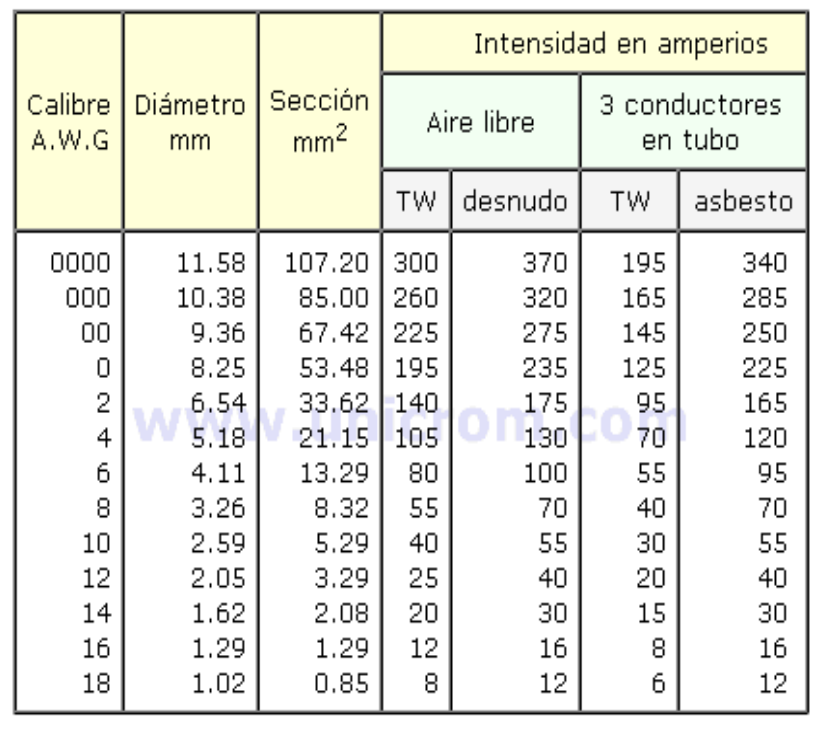
\includegraphics[scale=0.4]{conductorCobre.png}}
	\caption{Capacidades en conductores de cobre}
\end{figure}

\begin{figure}[ht!]
	\centering
	\fbox{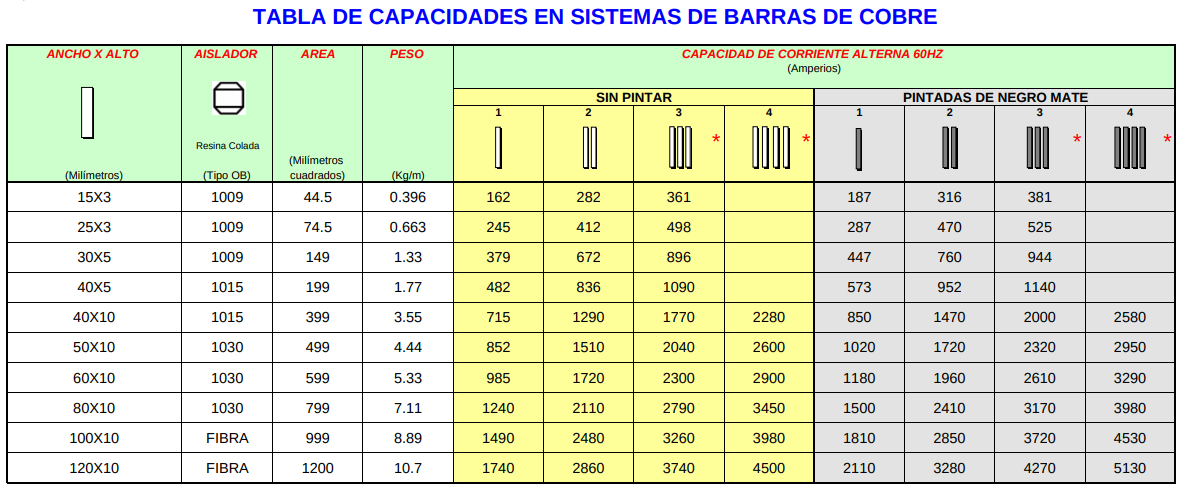
\includegraphics[scale=0.4]{barrasCobre.png}}
	\caption{Capacidades en Barras de Cobre}
\end{figure}
 
\end{document}
